% !TEX root = ../main.tex
% !TEX program = XeLaTeX
% !TEX encoding = UTF-8 Unicode

\date{2018년 3월 28일}

\begin{frontmatter}
\title{빠꼬어}
\author{김성}
\address{한국외국어대학교 베트남어과}
\begin{abstract}
Alves, Mark J. (2006). A grammar of Pacoh: a Mon-Khmer language of the central highlands of Vietnam. Pacific Linguistics, Research School of Pacific and Asian Studies, The Australian National University, 26--53.
\end{abstract}
\end{frontmatter}

%%%%%

\section*{발제 범위 분배}
\begin{table}[h]
\begin{center}
\def\arraystretch{1.5}
\begin{tabular}{>{\sffamily}ccccl}
\hline
	&\itshape 발제자	&\itshape 발제 범위		
	&\itshape 페이지	&\itshape 내용\\
\hline
1 & 김성 & Ch. 1-2 & pp. 1-15 & 서론, 음운론($\sim$이중모음) \\
2 & 김성 & Ch. 2-3 & pp. 15-33 & 음운론($\sim$차용어 음운론), 형태론($\sim$명사 형태론) \\
3 & 김성 & Ch. 3-7 & pp. 33-57 & 형태론($\sim$중첩어), 기본 구 구조 개괄, 부사, 접속사, 명사($\sim$보통 명사) \\
4 & & Ch. 7 & pp. 57-78 & 명사 \\
5 & & Ch. 8-10 & pp. 79-103 & 전치사, 문장 소사, 기본 동사 \\
6 & & Ch. 11 & pp. 106-111 & 보조 동사, SVC, VCT 동사 \\
\hline
\end{tabular}
\end{center}
\end{table}


\setcounter{section}{5}

\section{접속사}
어휘적인 표지 없이 병렬하는 것이 빠꼬어에서는 흔하지만 몇 가지 접속사가 가, 교체, 대조를 나타내기 위해 쓰인다. 접속사는 연결짓는 대상에 따라 동시 발생에 제약이 생긴다.

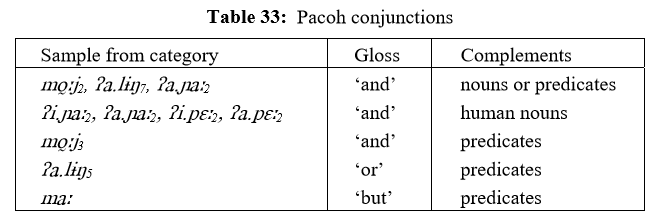
\includegraphics{Pacoh/src/PacohTable33.png}

\subsection{첨가 접속사 (`and')}
명사를 술어가 아니라 주어나 목적어로서 연결짓는다. ʔa.lɨŋ 은 `with'이라는 전치사와 동음이다. 이 전치사는 보통 주어에만 함께 쓰이지만, 접속사는 주어나 목적어에 좀더 자유롭게 나타날 수 있다.
S69, 70, 71 \omission

\subsection{인칭 접속사 (`and')}
인칭 접속사는 보어로 인간 명사만을 취한다. 이 종류에 속하는 모든 접속사가 빠꼬어의 이음절 대명사와 동음이고, 관계된 형태와 의미 자질을 공유한다.
이 접속사들은 2인칭이나 3인칭인 둘 이상의 보어를 취한다.

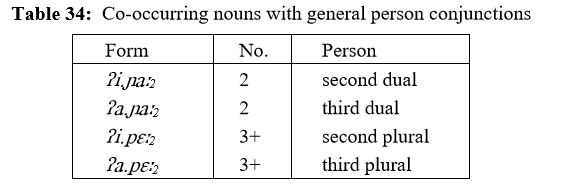
\includegraphics{Pacoh/src/PacohTable34.png}

이상의 형태는 단수 명사와 의미적으로 복수인 명사의 조합도 취할 수 있다. 이는 수와 인칭 요인의 의미적 일치이다. 보어에게 요구되는 자질은 동음의 대명사 형태의 자질과 일치한다. S. Watson (1964)

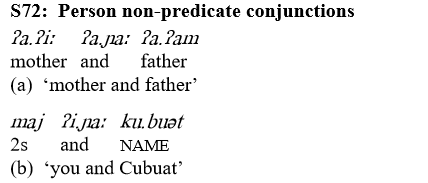
\includegraphics{Pacoh/src/PacohS72.png}

97년에 16세에서 20세 사이의 빠꼬 화자들로부터 채록한 자료에서는 ʔa.ɲaː가 명사의 인격성이나 보어의 수에 대한 고려 없이 쓰였다. S73에서 이 접속사는 사람이 아닌 보어를 취하고 있고 S74에서는 2개의 복수 보어를 취하고 있다. 여기에서 이 접속사는 비인격 비술어 접속사(non-person non-predicate-taking conjunction)로 여겨지는 것이다. 이것이 지역적 변이로 밝혀지지 않는다면, Watson이 기술한 접속사 패러다임은 소실되어가는 중일 수 있고 ʔa.ɲaː는 표준 기본형 접속사가 되어가고 있다.

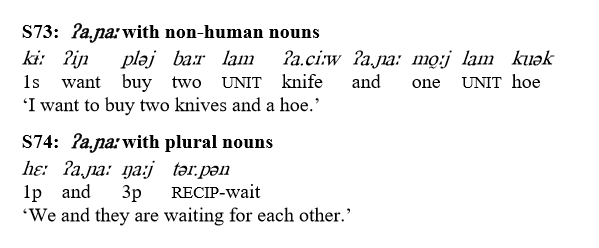
\includegraphics{Pacoh/src/PacohS73.png}

\subsection{술부를 취하는 첨가 접속사(`and')}
동사를 이을 때는 병렬이 흔하지만 특히 두 동사가 연속적이라기보다 동시적일 때는 접속사 mo̰ːj가 가끔 쓰인다.

\subsection{대체 접속사(`or')}
\omission

\subsection{대조 접속사(`but')}
빠꼬어의 유일한 대조 연장 접속사(contrary extension conjunction)는 maː `but'이다. 주로 두 동사 사이에 오지만 명사 술어도 취할 수 있다.

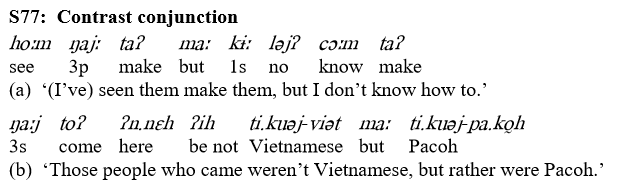
\includegraphics{Pacoh/src/PacohMaExample.png}


\section{명사}
%넘어가도댐
\subsection{보통 명사}
%여기서부터시작
동남아의 다른 종별사 언어에서와 마찬가지로 보통 명사는 대부분 불가산명사이다. 보통 명사는 의미적, 통사적 일치를 보이는 종별사나 단위명사를 수반해야만 수량을 나타내는 명사구(quantified noun phrases)에 나타날 수 있다.
보통 명사는 복수성이나 특정성(definiteness)가 정해져 있지 않으므로 그러한 자질을 나타내는 수량 명사나 한정사와 같은 단어와 함께 나타난다. 또는 담화 맥락으로 나타나기도 한다. 다른 표지가 없는 보통 명사는 복수 상태 동사나 상호 동사 등을 수반하면 복수인 것으로 해석할 수 있다.

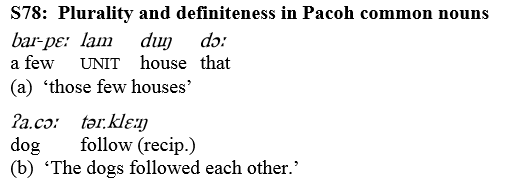
\includegraphics{Pacoh/src/PacohS78.png}

담화 맥락이나 한정사가 없을 경우 보통 명사는 정해진 가산적 단위를 가리키기보다 부정(indefinite)적인 집합을 가리킬 수 있다.

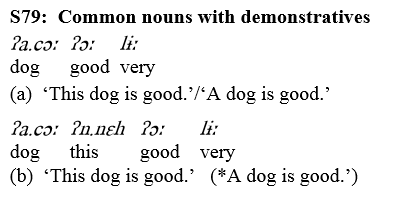
\includegraphics{Pacoh/src/PacohS79.png}

\subsubsection{일반적인 보통 명사}

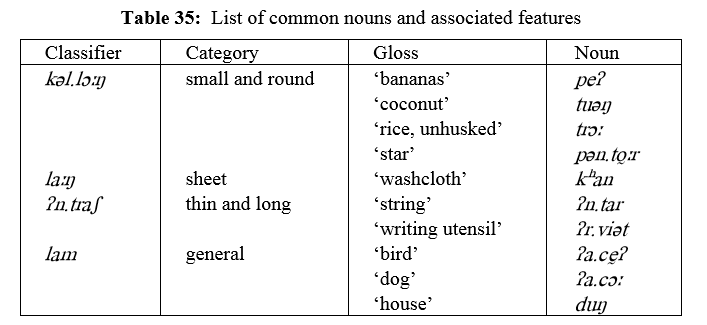
\includegraphics{Pacoh/src/PacohTable35.png}

명사의 자질과 종류에 따라 붙을 수 있는 종별사에 제한이 있다. 

3.1.5에서 소개한 시간 표현 명사는 보통 명사이지만 이미 의미적으로 숫자를 나타내는 자질이 있기 때문에 수량화된 명사구에 나타나지 못한다. `day', `year', `time' 등 시간 단위 명사와는 별개이다. (7.2.2, 12.7 참조)

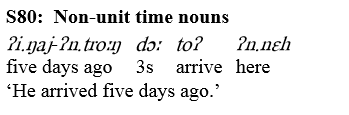
\includegraphics{Pacoh/src/PacohS80.png}

\subsubsection{인간 보통 명사}
\begin{itemize}
\item 가족 관계, 연령 그룹, 직업, 민족 그룹 등 다양한 의미장 내의 어휘들을 포함한다.
\item 인간 종별사 단위 명사, 인간 접속사와 같이 쓰인다.

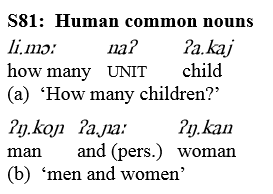
\includegraphics{Pacoh/src/PacohS81.png}

\end{itemize}

\subsubsection{집합(mass) 보통 명사}
수 표지나 특정성 표지가 없는 보통 명사는 의미적, 통사적으로 집합 명사의 성질을 지닌다.
그러나 특정 명사들은 일반적인 의미적 자질 때문이 아니더라도 집합 명사의 범주에 속한다.
집합 보통 명사는 ti.ŋaːn `bowl' baːw `bag' ʔa.tɛːh `basket' 등 종별사가 아닌 가산 단위 명사와는 함께 쓰이지만 종별사 단위 명사와는 쓰이지 않는다.

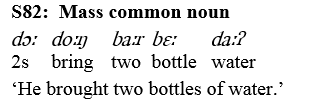
\includegraphics{Pacoh/src/PacohS82.png}

일부 비-집합 명사 중에는 집합명사처럼 기능할 수 있는 단어가 있다. 이들은 주로 집합적인 측량 단위에 보관된다. S83(a) 에서 `바나나'는 단일 단위이지만 S83(b)에서는 바구니의 내용물을 가리킨다.

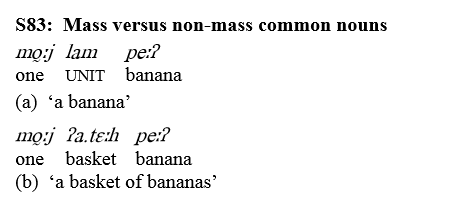
\includegraphics{Pacoh/src/PacohS83.png}

\subsubsection{발화 명사 절}
여기서 하나의 통사적 성분으로 나타낸 발화 명사 절은 발화 동사(speech verbs)의 명사적 보어이다.

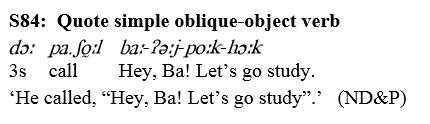
\includegraphics{Pacoh/src/PacohS84.png}

\subsubsection{고유 보통 명사}
\begin{itemize}
\item 고유 보통 명사는 주로 인명 이외의 다양한 명칭(non-human names), 지명, 민족명 등을 포함한다.
\item 고유 보통 명사는 특수한 독립체로서 수량화된 명사구에서 단위명사 뒤에 나타나지 않는다. 
\item 고유 대명사(7.3.4)는 고유 보통 명사와 다르게 일반적으로 사람 또는 최소한 사람과 같은 성질이 있는 유정(animate) 명사에 대한 지칭에 쓰이고 인간에 관련된 대명사적 자질을 갖는다.
\item 주어진 데이터에서 고유 명사의 예는 ʔa.lɨəj `아르어이(빠꼬인들이 많이 사는 곳의 지명)' miːʔ `미국' 등이 있다.
\end{itemize}

\subsubsection{의미적으로 일반화된 합성 명사}
의미적으로 일반화된 합성 명사는 3.3.1에서 소개된 절 결합에 참여할 수 있는 다음절 어휘의 집합을 이룬다.
이러한 명사들은 의미영역이 겹치는 둘 이상의 어휘와 유사하고 공통의 일반화된 의미 영역을 나타내는 음운론적 소재를 포함한다. 예를 들어 jəw-baːj `friends (in general)' 는 각각 `친구'라는 의미를 가진 두 별개의 어휘와 음운론적 소재를 공유한다. duŋ-vḛːl `society'는 각각 `집'과 `마을'의 음성적 형태로 이루어져 있다.
절 중첩에 대한 자료는 R. Watson (1966b and 1980) 에 제공되어 있다.

S85에서 합성어 `literate'은 동사 cɔːm `알다'와 일반화된 중첩 명사 ʔu.raʔ-ʔu.ʔar `글(writing)'을 포함한다.

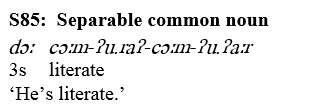
\includegraphics{Pacoh/src/PacohS85.png}

이러한 명사는 수사 명사나 단위 명사의 종속어(dependents)로 나타나지 않고 다른 단어를 종속어로 취하지도 않는다. 이러한 수 및 한정성의 부재가 이 단어들의 의미적 포괄성(generic semantic nature)을 두드러지게 한다.